\documentclass[a4paper, 12pt]{article}
% math symbols
\usepackage{amssymb}
\usepackage{amsmath}
\usepackage{mathrsfs}
\usepackage{physsummer}


\usepackage{enumitem}
\usepackage[margin = 2cm]{geometry}

\tolerance = 1000
\emergencystretch = 0.74cm



\pagestyle{empty}
\parindent = 0mm

\begin{document}

\setphysstyle{ГЦФО 8}{Серия Ш-08}{09.11.2016}

\large
\setcounter{notask}{24}

\taskpic{ Экспериментатор взял 4 одинаковых металлических стержня и
  собрал из них Y-образную фигуру. К концам фигуры экспериментатор
  присоединил 3 одинаковых больших металлических шара, имеющих
  температуру $t_1=0^{\circ}$C, $t_2=50^{\circ}$C и $t_3=100^{\circ}$C
  (см. рис.). Экспериментатор обеспечил хороший тепловой контакт
  стержней с шарами и другими стержнями. Через некоторое время он
  обнаружил, что первый шар нагрелся на $0{,}4^{\circ}$C. Какую
  температуру имели в этот момент два других шара?  Считайте, что
  теплоёмкость стержней пренебрежимо мала, а теплообмен с окружающей
  средой отсутствует. Мощность теплопередачи по стержню
  пропорциональна разности температур на его концах. }
{
  \begin{tikzpicture}[circuit ee IEC]
    \node[contact] (A) at (0,0) {};
    \node[contact] (B) at (0,-1) {};
    \node[contact] (C) at (0,-2) {};
    \node[contact] (D) at ($(A)+(45:1cm)$) {};
    \node[contact] (E) at ($(A)+(135:1cm)$) {}; 
    \draw[thick] (D) -- (A) -- (B) -- (C);
    \draw[thick] (E) -- (A);
    \draw[thick] (D) ++ (45:0.5cm) circle (0.5cm) node {2};
    \draw[thick] (E) ++ (135:0.5cm) circle (0.5cm) node {1};
    \draw[thick] (C) ++ (0,-0.5cm) circle (0.5cm) node {3}; 
  \end{tikzpicture}
}

\taskpic{Три одинаковых источника тепла расположены в цилиндре,
боковые стенки и один из торцов которого теплоизолированы. Второй
торец цилиндра закрыт теплопроводящей мембраной. При наружной
температуре $t_0 = 10^\circ$C в цилиндре устанавливается температура
$t = 25^\circ$C. В цилиндр помещают еще две такие же мембраны,
отделяющие источники друг от друга. Какие температуры установятся в
образовавшихся секциях? Считайте, что мощность теплопередачи
пропорциональна разности температур. Температуру воздуха в пределах
каждой отдельной секции (а до установки дополнительных мембран --- во
всем цилиндре) считайте
одинаковой.}{
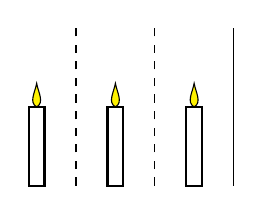
\begin{tikzpicture}
  \platform{(3,0)}{(0,0)};
  \platform{(0,-0.15)}{(0,2.15)};
  \platform{(0,2)}{(3,2)};
  \draw (3,0) -- (3,2);
  \draw[dashed] (1,0) -- (1,2);
  \draw[dashed] (2,0) -- (2,2);
  % свечи
  \draw[thick] (0.4,0) rectangle ++(0.2,1);
  \draw[thick] (1.4,0) rectangle ++(0.2,1);
  \draw[thick] (2.4,0) rectangle ++(0.2,1);
  % пламя
  \draw[fill=yellow] (0.5,1) to[out=30,in=-80] (0.5,1.3) to
  [out=-100,in=150] (0.5,1);
  \draw[fill=yellow] (1.5,1) to[out=30,in=-80] (1.5,1.3) to
  [out=-100,in=150] (1.5,1);
  \draw[fill=yellow] (2.5,1) to[out=30,in=-80] (2.5,1.3) to
  [out=-100,in=150] (2.5,1);
\end{tikzpicture}
}


\end{document}


%%% Local Variables: 
%%% mode: latex
%%% TeX-engine:xetex
%%% TeX-PDF-mode: t
%%% End:
